\resetfigpath{1-intro}

\chapter{Introduction}
\label{intro}

The medical imaging field has recently witnessed the revolution of \gls{ai}, a broad discipline that is a part of computer science whose aim is to conceptualize human ``intellectual'' tasks, and produce computer programs that can replicate them, thereby allowing to relieve human beings from tedious and repetitive tasks.
From classification to segmentation tasks, \gls{ai} already provides flexible and efficient tools that greatly facilitate the daily practice of clinicians.
In particular, large quantities of \gls{mri} brain scans are now efficiently and accurately processed by \gls{ai} systems that help clinicians in the diagnosis of pathologies \cite{sun19}.
Similarly, surgical instruments can be segmented automatically and accurately in real-time to allow laparoscopic interventions of the abdominal cavity by means of robotic technology, thereby decreasing the invasiveness of traditional methods \cite{davinci}.

\Gls{ml}, a term that denote a sub-category of \gls{ai}, is grounded on the ``learning by example'' paradigm.
Whereas traditional approaches generally consisted in explicitly formalizing and implementing complex tasks as a combination of simpler programmatic instructions,
\gls{ml} rather considers that a flexible system can learn such instructions automatically through repeated experiences.

Concretely, as a young child can effectively derive the concept of car using a few visual examples, and be able to identify an ``unseen'' car in a complex environment with near-perfect accuracy,
state-of-the-art \gls{ml} methods leverage the same principle.
However, no matter how well-engineered they are, they need, in order to replicate this simple task with comparable accuracy, thousands of examples and counter-examples of images \cite{ILSVRC15}.

In this scenario, collecting such quantity of example images and annotating them is tedious and cumbersome.
In practice, the annotation task is performed by numerous individuals in parallel.
The annotation of medical data, however, adds the following practical difficulties.
First, the task can require a specific medical expertise.
Second, assuming such experts are available and willing to participate to this task, their daily obligations imposes a limited time budget.
These two factors largely explain why the medical field does not benefit from the latest and greatest \gls{ml} technologies used in more generic applications \cite{orting19}.


\section{Proposed annotation protocol and applicability}

In the present thesis, we devise solutions that allow to annotate medical sequences in a fast and intuitive manner, in an attempt to alleviate the bottleneck of scarcity of example data.

In particular, the annotator is presented a video or volumetric sequence that plays on a screen, i.e. the frames unfold in an automatic manner.
As the sequence unfolds, the annotator is asked to point at the object of interest using a pointing device, such as a mouse, a tablet pen, or an eye-gaze tracker.
In contrast with the traditional approach, where the object must be manually segmented on each frame individually, the proposed protocol drastically reduces the annotation time.
In essence, our contribution ambitions an annotation time equal to the duration of the video/volume playback.
For example, assuming the sequence contains $100$ frames playing at $5fps$, the total annotation time is $20$ seconds.
In comparison, the traditional pixel-wise annotation task of a sequence of similar size could take anywhere from $10$ min. to $1$ hour.

Concretely, we set the following requirements on the annotation protocol:
\begin{itemize}
  \item The annotator does not need to manually change the frame being annotated, e.g. by hitting a forward or backward key. The sequence automatically unfolds according to a specified frame-rate.
  \item The annotator handles a single pointing device, which he/she uses to indicate the location of the object of interest.
  \item The annotator must be able to watch and annotate the sequence in a single go, i.e. he/she does not need to review annotations and modify them manually afterwards.
\end{itemize}

The segmentation method must be functional in a variety of situations, namely produce acceptable accuracy for:
\begin{itemize}
  \item Both videos and volumetric sequences.
  \item Both color and grayscale images.
  \item Various kind of image modality, e.g. \gls{mri} and \gls{ct}.
  \item Various levels of noise, perturbations, and lightning artifacts.
  \item Various nature of object, i.e. size, shape, appearance.
  \item The object can be made of several parts that are not immediately contiguous, i.e. an \gls{mri} brain scan with several tumors.
\end{itemize}

\section{Datasets}

We now introduce the datasets that have been used during the elaboration and testing of the proposed solutions.
Note that as the range of possibilities is huged, we chose to restrict ourselves to $4$ types of sequences. These, however, cover the entirety of the proposed spectrum.

In particular, we now describe them in detail and give each type a short name that will be used in the remaining of this thesis:

\begin{itemize}
  \item \textbf{Tweezer}: Surgical instruments during an endoscopic procedure, where the instrument is object of interest.
    The background is relatively homogeneous, while the instrument moves accross the frame both in translation and rotation.
    The sequences are taken from the MICCAI EndoVision Challenge \cite{EndoChall}.
    Each sequence is around $120$ frames long, i.e. represent $\sim 5s$ of video acquired at $25$ fps.
  \item \textbf{Cochlea}: Volumetric \Gls{ct} scans of the inner-ear where the cochlear labyrinth is to be segmented. These are acquired according to different protocols, and therefore show important variations in gray-scale level, orientation, as well as sizes. Furthermore, the object of interest is composed of different parts that split and merge.
  \item \textbf{Slitlamp}: Microscopic video of the retina where the optic nerve is to be segmented. The videos have been acquired using a slitlamp instrument.
    The optic nerve is of rather small size. The background often shows important artifacts, in the form of yellow and blue beams, which sometime overlap with the object of interest. The movement of the optic nerve is often very jerky.
  \item \textbf{Brain}: Transverse \gls{mri} scans of brains where the tumor is object of interest. The sequences are taken randomly from the Brain Tumor Segmentation Challenge (BRATS) public database \cite{BRATSChall}.
    Scans are acquired using the same \gls{mri} protocol, but with different scanners, thereby showing wide variety of contrast and color.
    The tumors have varying size, colors, and shapes. Sometimes, the same scan shows several tumors on the same slice.

\end{itemize}

In Fig. \ref{fig:dset_previews}, we show example frames for each type.

\begin{figure}
\centering
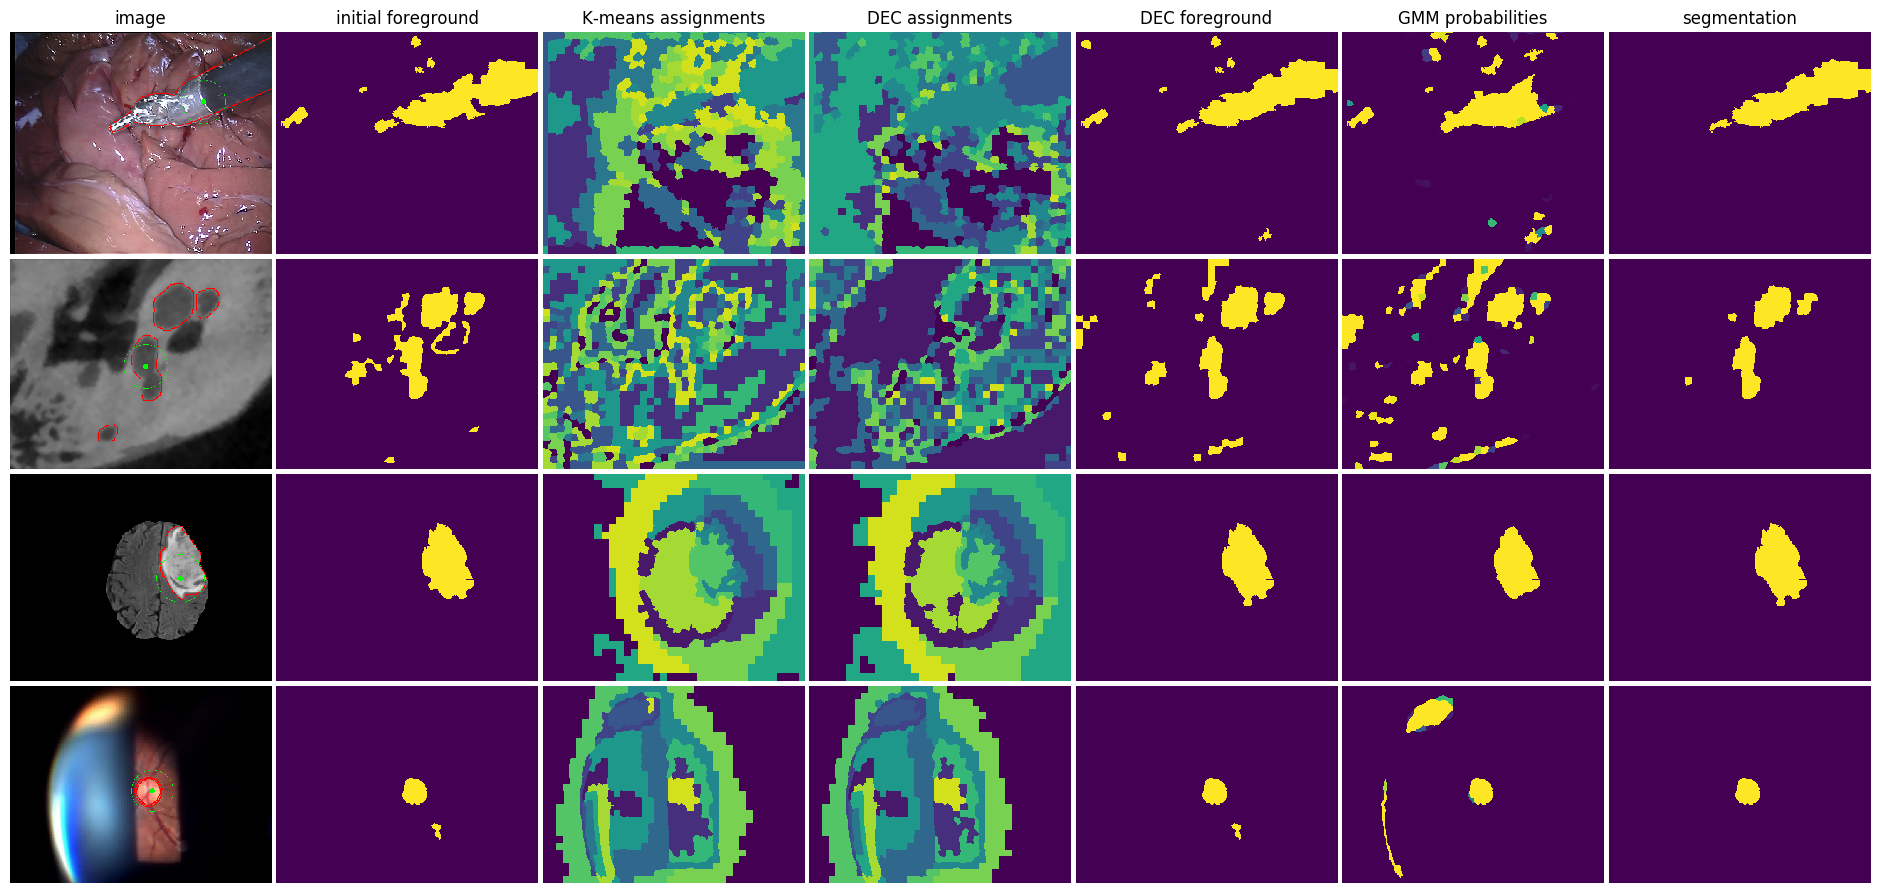
\includegraphics[width=0.99\textwidth]{prevs.png}
\caption{Example of objects of interest in different video and volumetric modalities. Each type contains 4 sequences. We show a single frame per sequence.
  From top to bottom: Tweezer, Cochlea, Slitlamp, and Brain}
\label{fig:dset_previews}
\end{figure}

\section{Annotation Software and Web Platform}
In the frame of this thesis, a flexible and elegant annotation software was developed that supports as pointing device a traditional mouse, a pen compatible with touch-screens, as well as an interface to connect a eye-gaze tracker through the USB port.
Also, a web interface was designed and implemented that allows a user to upload a sequence annotated using the above software, and download the generated pixel-wise segmentation when they are ready.
We now describe both contributions.

\subsection{Sequence annotation tool}
\label{sec:anna}

The typical annotation workflow is as follows:

\begin{enumerate}
  \item[-]{Provide as input a volume/video. These can be either DICOM \cite{dicom}, or video files.}
  \item[-]{Optional: Set the framerate at which the sequence will play (right knob on Fig. \ref{fig:anna}).}
  \item[-]{Optional: Connect the software to the eye-gaze tracker server. The tracker will then act as a secondary mouse.}
  \item[-]{Hit the play button. The sequence unfolds.}
  \item[-]{Give point annotations:}
    \begin{itemize}
      \item[-]{When using mouse: Simply click on the desired region.}
      \item[-]{When using gaze-tracker: Place gaze on region and use right button (Fig. \ref{fig:anna}) to activate the recording of locations.}
    \end{itemize}
  \item[-]{Save locations in \gls{csv} file.}
\end{enumerate}

\begin{figure}[!htpb]
  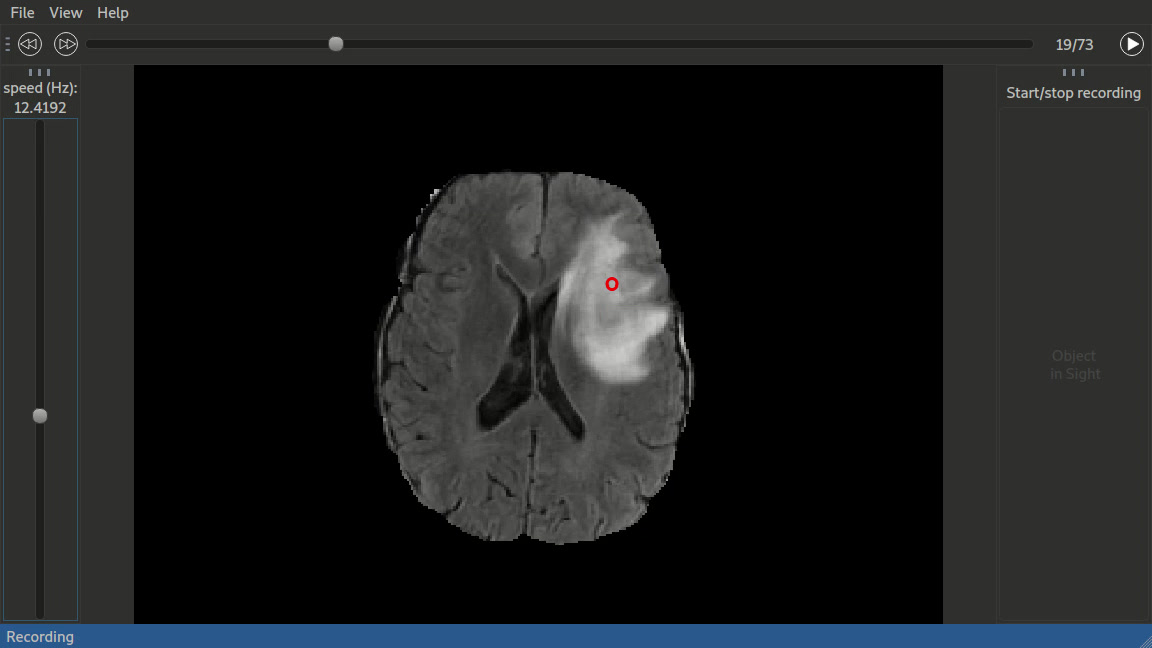
\includegraphics[width=0.99\textwidth]{anna0.png}
  \caption{Screenshot of annotation tool. }
  \label{fig:anna}
\end{figure}

The software is intended to be cross-platform and be compatible with a variety of input formats.
Second, as our early experiments relied on an eye-gaze tracker, our software needed to be compatible with the proprietary backend given by the manufacturer.
Third, a simple \gls{gui} was needed to display images and allow the user to select his favorite modality of annotation.
The latter requirements drove our choice towards the Qt5 framework \cite{eng16}, which relies on C++ and provides convenient widgets out of the box.
Our software supports allows to annotate using a mouse and an eye-gaze tracker \cite{eyetribe}.
As platform, it supports the Linux, MacOS and Windows operating systems.
We provide the source code at \href{https://github.com/aimi-lab/Anna}.

\subsection{Web platform}
The segmentation methods presented in the next chapters require important computational resources, namely a \gls{gpu} to train deep networks.
We therefore provide a way for users to upload their data along with the corresponding 2D locations to a server that will perform the necessary computations remotely and send back segmentation results when they are available.
Concretely, we develop a web interface that provides:

\begin{itemize}
  \item[-]{Links to download the annotation software (Sec. \ref{sec:anna}).}
  \item[-]{A login mechanism that provides us with a contact e-mail address.}
  \item[-]{An upload form where the user drops his sequence along with the 2D locations}
\end{itemize}

Once the data has been uploaded, a task object is created and queued until computational resources are available.
After completion, the user is warned that he can download his segmentations via a URL.

\begin{figure}[!htpb]
  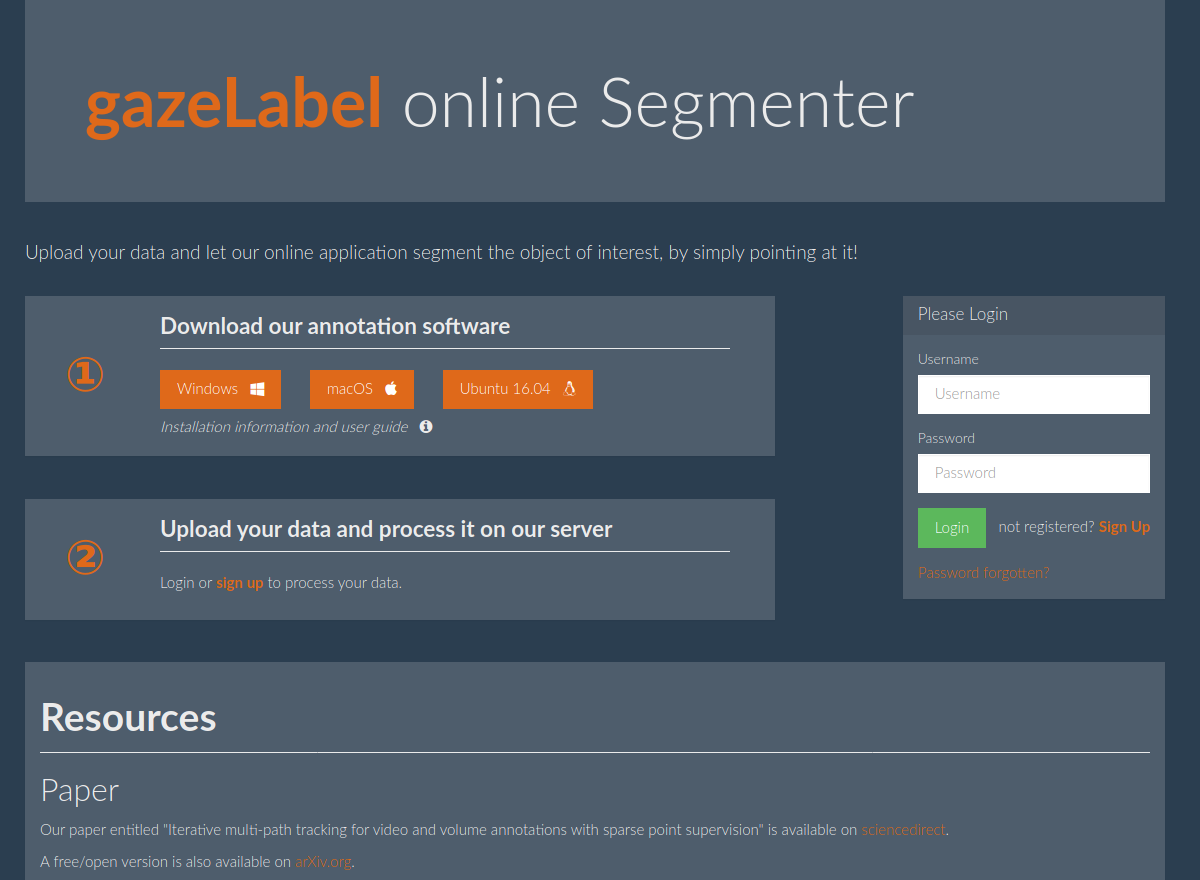
\includegraphics[width=0.99\textwidth]{gazelabel.png}
  \caption{Screenshot of our web platform. Home page.}
  \label{fig:anna}
\end{figure}

The frontend, which generates the web pages uses the \href{https://webpack.js.org}{Webpack} bundler.
The backend is based on the \href{https://www.djangoproject.com/}{Django} framework, which handles different applications, namely the forms (login, data upload), the job queue, and the database.

\begin{figure}[!htpb]
  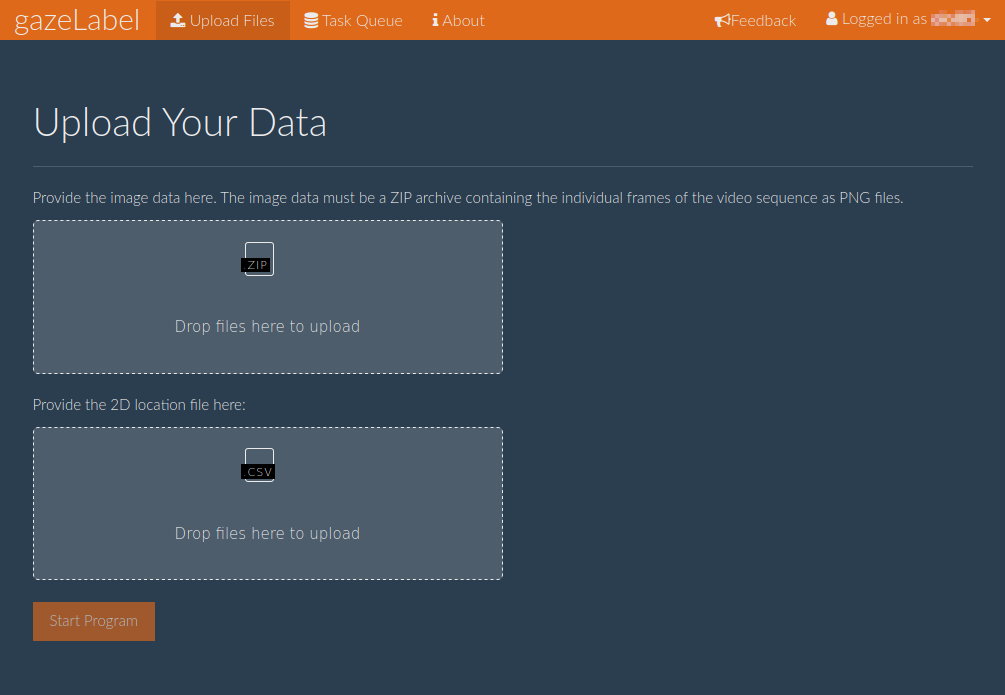
\includegraphics[width=0.99\textwidth]{gazelabel_upload.png}
  \caption{Screenshot of our web platform, where the user can upload a sequence and its corresponding annotations. The task queue panel shows the state of the submitted tasks.}
  \label{fig:anna_upload}
\end{figure}



\section{Related Works}

Past research that address this issue can be roughly divided in two categories,
where the first leverages computer vision techniques to generate segmentation masks from sparse and/or noisy annotations, while the second focuses on developping Machine Learning techniques to minimize an annotation budget.
In practice, both categories often overlap.

We start by giving an overview of state-of-the-art in computer vision.
Next, we focus on \gls{ml} methods.
In particular, we emphasize on domains that target segmentation in a semi-supervised setting.

\subsection{Computer Vision Methods}
Another line of research focuses on the annotation protocol itself so as to complement the above efforts.
While the most tedious protocol requires that images be manually segmented at a pixel-level, many computer-vision approaches exist to facilitate this task.

Early contributions relied on the Active Contour model \cite{kass88}, which assumes that an initial contour is given and parameterized as the nodes of a spline curve, in this context called an elastic snake.
The segmentation problem is formulated as finding the deformation of the initial snake that minimizes an energy term.
In its simplest form, the energy term is composed of a term that determines the fitting of the snake to the edges of the image, while another term controls the smoothness of the snake.
The energy is then minimized using gradient descent.
Following works alleviate the problem of robustness brought by noisy edge maps by minimizing the Mumford-Shah functional \cite{chan01}, and parameterize the contour using the level-set method \cite{osher88}.

More recently, annotations in the form of scribbles were considered, where the annotator is asked to draw crude delineations of one or several objects of interest, along with a scribble on the background.
A first method that handles such kind of annotations relies on the Random-Walk algorithm \cite{grady06}.
The segmentation problem reduces to assigning to each unlabeled pixel a random-walker. The label of the latter pixel is then determined by the finding the label for which the walker has a maximum probability of reaching first.

Relying on the same annotation requirement, the graph-cut approach \cite{Boykov2006}
minimizes an Markov Random Field energy objective that considers unary terms (a scalar on each pixel), and a pairwise term that models the similarity of neighboring pixels.
Concretely, the image or volume is represented as a region adjacency graph where each pixel is assigned a node, and edges connect adjacent pixels.
Each annotated positive pixels is connected to a source node, while annotated negatives are connected to a sink node.
The energy minimization is then performed using the min-cut/max-flow algorithm \cite{goldberg88}.
Using the same algorithm, grab-cut \cite{rother04}, further simplifies the scribble-based annotation protocol by considering bounding-boxes around the object of interest, which provide crude labels on both foreground and background in a single stroke.

Along the same line, \cite{criminisi08}

\subsection{On the Wise Use of Annotation Budget}
The problem of scarcity of labeled data can also be posed in the following manner:
Given a limited annotation budget, i.e. when only a few hours of annotation work can be provided, how can one make the best use of it?

\gls{al} \cite{settles09} considers semi-supervised learning scenarios, where abundant unlabeled data are available.
\gls{al} algorithms select unlabeled samples that are the most informative to the \gls{ml} model, i.e. it assumes that many unlabeled samples represent redundant information to the late-stage \gls{ml} model.
In \cite{KonSznFua15}, authors devise a strategy to select unlabeled supervoxels of a 3D volume so as to segment volumes of various modalities.
The approach iteratively trains a classifier and takes its entropy as measure of uncertainty.
Combining the latter with a geometric prior, which takes into account intuitive rules on spatial coherence, they sample a batch of most uncertain samples.
The classifier is then re-trained using the newly annotated samples.

Crowd-sourcing, refers to the outsourcing of the annotation task to a high number of annotators \cite{orting19}.
Its use in the frame of medical imaging poses several limitations.
First, the difficulty of the annotation task can prohibit the effective use of crowd-sourcing, e.g when the structure of interest is hard to distinguish \cite{orting19}.
Another limitation is the nature of the data, i.e. one usually prefers to pre-classify brain scans and submit to workers the slices where tumors are present.
Last, one must usually integrate a test-task to ensure the competence of workers, or filter-out annotations provided by ``poorly performing'' workers \cite{park18}.

\subsection{Transfer Learning, Semi-supervised Learning, and Domain Adaptation}
\gls{tl} consists in using a \gls{ml} model trained for the task of interest, but using a training set of different nature than the targeted domain, e.g. train a \gls{cnn} to segment natural objects (trees, cars, ...) for the segmentation of surgical tools.
As pointed out by \cite{oliver18}, an important and implicit assumption in that context is that both datasets share similar data distributions.

\gls{ssl} is a broad category of \gls{ml} algorithm that combines traditional supervised learning tasks, where a fully labeled training dataset is available, along with an abundant unlabeled dataset.
The latter can, under specific conditions, boost the performance of an \gls{ml} model trained with labeled dataset only, i.e. in a fully-supervised manner.
The basic idea is that the ML model may acquire knowledge of the data distribution from the unlabeled set.
Here again, one assumes that both data domains share similar distributions.
In \cite{ghafoorian17}, authors show experimentally that a \gls{nn} trained to segment tumors on MRI brain scans acquired in a given MRI protocol, perform poorly when transfered to another protocol, as the shape, intensities, and contrast level are inconsistent.

\gls{da} addresses the problem of adapting the model so as to take into account domain shift, i.e. the discrepancies between the training and target domain.
In \cite{perone19}, authors devise a strategy to segment MRI scans of spinal cords using a model trained with images taken at a specific field-of-view, and transfer to another field-of-view in an unsupervised fashion.
Their approach leverages data-augmentation to enforce a consistency between the augmented and pristine images of the unlabeled set, while jointly training with the labeled set with traditional cross-entropy loss.
On the same image modality, \cite{li20} resort to adversarial training. They jointly train a segmentation model and a discriminator wit shared weights. The discriminator is trained to discriminate between the source and target domain.





%%% Local Variables:
%%% mode: latex
%%% TeX-master: "../../main"
%%% End:
